% !TeX spellcheck = sk_SK
 

  

\section{Analýza problému} 

  

\subsection{Úvod do petriho sietí} % not called Petriflow 

 Petriho siete sú modelovací nástroj určený na modelovanie udalostných systémov. 

% TODO - skopcit od milana .. 

  

  

\subsection{Procesný server} 

 Majme procesný server tento server v sebe obsahuje informáciu o rôznych procesoch. Tieto procesy majú rôznu štruktúru a sú v rôznych stavoch. Štruktúru týchto procesov môžeme reprezentovať pomocou Petriho sietí a ich stav pomocou rôznych značkovaní v týchto sieťach.  

% TODO - najprv odstavec pred tým 

  

\subsection{Aplikačné rozhranie} 

 Na to aby sme mohli k dátam pristupovať zvonka uzavretej domény procesného servera potrebujeme vytvoriť aplikačné rozhranie ktoré bude riešiť autentifikáciu, autorizáciu a dokumentáciu.  

% TODO 

  

  

  

  

\section{Špecifikácia} 
V tejto kapitole najprv stručne opíšeme hlavnú funkcionalitu navrhovanej aplikácie, potom zadefinujeme funkcionálne a nefunkcionálne požiadavky na aplikáciu. 

Softvér, ktorý sme sa rozhodli implementovať bude slúžiť ako rozhranie medzi procesným serverom a internetom. Bude umožňovať klientovi pripojiť sa na procesný server cez internet, získať informácie o dátach v prechodoch petriho siete a bude umožňovať modifikovať stav siete (procesu) spúšťaním prechodov.  
\cite{t01} sdkjjsad
  

\subsection{Funkcionálne požiadavky} 

\begin{enumerate} 

    \item Rozhranie bude umožňovať registrovať používateľov a priraďovať im roly 

    \item Umožní prihlásenie používateľa pomocou štandardného autentifikačného protokolu. 

    \item Autentifikovaným používateľom umožní prístup k dátam z tých prechodov ktoré majú právo čítať podľa ich roly. 

    \item Autentifikovaným používateľom umožní spúšťať prechody ktoré majú právo spúšťať podľa ich roly. 

    \item Pri spúšťaní prechodu prebehne validácia vstupných dát. V prípade nevalidných alebo nekompletných dát nepovolí spustenie prechodu. 

    \item Rozhranie poskytne online dokumentáciu prechodov v sieti, táto dokumentácia bude zahŕňať URL prechodu, potrebné dátové polia na spustenie prechodu a roly, ktoré sú oprávnené prechody spúšťať. 

    \item Rozhranie poskytne aplikačné rozhranie viacerým sieťam s rôznou štruktúrou. 

\end{enumerate}     

  

 
  

\subsection{Nefunkcionálne požiadavky} 

\begin{enumerate} 

    \item Rozhranie bude škálovateľné 
    \item Rozhranie bude napísané vo frameworku Spring Boot 
    \item Rozhranie bude zabezpečené štandartnými bezpečnosntými prvkami
	
\end{enumerate} 

  

\section{Návrh} 


% TODO - what have we done in this chapter? 

 

\subsection{Prípady použitia}
Zo špecifikácie vyplývajú nasledovné interakcie používateľa s naším systémom.

\subsubsection{Registrácia koncového bodu}
Prvý prípad použitia \ref{usecase1} je registrácia koncového bodu. Aktér ktorý môže registrovať koncové body je len administrátor. Pri tejto akcií administrátor poskytne nášmu systému informácie o štruktúre procesu vo formáte petriflow, zoznam používateľov im prislúchajúcich rolí v XML a unikátny identifikátor siete. Pokial che administrátor upraviť spustí proces registrácie nanovo s upravenými údaji o sieti.

Administrátor taktiež môže sieť vymazať. \ref{usecase1}
\begin{figure}[!htbp]
	\centering
	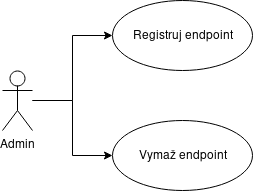
\includegraphics[width=6cm]{img/dp_usecase_1_register.png}
	\caption{Prípad použitia - Registrácia koncového bodu}
	\label{usecase1}
\end{figure} 

\subsubsection{Získanie informácie o prechode}
Keď už sú sieť aj používateľia úspešne zaregistrovaný, si môžu používatelia, vyžiadať \ref{usecase2} informácie o prechode. Tieto informácie budú poskytnuté len používateľovi s rolou oprávnenou na čítanie dát z daného prechodu.

\begin{figure}[!htbp]
	\centering
	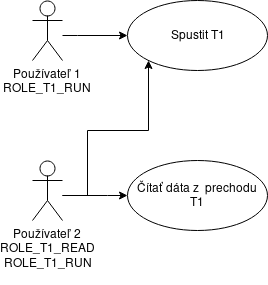
\includegraphics[width=6cm]{img/dp_usecase_2_read_run.png}
	\caption{Prípad použitia - Získanie informácií o prechode}
	\label{usecase2}
\end{figure} 

\subsubsection{Spustenie prechodu}
Používateľia s príslušnými rolami môžu taktie spúšťať \ref{usecase2} prechody. Pri spustení prechodu poskytne používateľ dátové polia potrebné na spustenie prechodu. 

\subsubsection{Autentifikácia}
Z požiadavky na bezpečnosť aplikácie vyplýva ešte prípad použitia, kedy sa neautentifikovaný používateľ autentifikuje, aby nadobudol identitu rozpoznanú našim systémom. 



\subsection{Architektúra} 

Aby sme splnili požiadavku na jednoduché škálovanie aplikácie a pre sprehľadnenie architektúry zvolili sme si architektúru mikroservisov. Táto architektúra pozostáva z viacerých oddelených častí, každá z týchto častí má svoju jasne definovanú funkciu. Takéto mikroservisy sú jednoducho testovateľné, dajú sa nasadzovať postupne a nezávisle od seba a softvér navrhnutý v tejto architektúre býva spravidla robustný a vysoko škálovateľný.  

Softvér sa bude skladať z troch hlavných služieb: generátor, koncový bod, autentifikačná služba
\begin{itemize}
	\item Generátor je služba, ktorá bude registrovať a zostavovať koncové body. Je to služba, na ktoú sa pripojí adiministátor, zadá štruktúru siete a zoznam používateľov a rolí. Táto služba následne zaregistuje používateľov a ich roly, vygeneruje kód pre službu koncového bodu a túto služnu spustí.
	\item Koncový bod je služba, ktorá obsahuje vygenerovaný kód koncových bodov. Táto služba bude poskytovať dokumentáciu dostupných konových bodov. bude poskytovať samotné koncové body aprizavolaní koncového bodu sa bude starať o validáciu prijatých dát.
	\item Autentifikačná služba sa stará o autentifikáciu používateľov a pridelovanie rolí použivateľom
	%TODO other containers
\end{itemize}

Okrem 



\section{Implementácia} 

% TODO 

  

\subsection{Použité technológie} 

  

\subsubsection{Kotlin} 

Kotlin je relatívne nový programovací jazyk, projekt Kotlin bol po prvý krát zverejnený v roku 2011 spoločnosťou JetBrains(Andrey Breslav). Bol vyvinutý ako moderný staticky typovaný jazyk, ktorý podporuje rýchlu kompiláciu do javy. V roku 2017 vyhlásil Google podporu pre Kotlin v operačnom systéme Android.  

Medzi jeho hlavné výhody patrí menší boilerplate (menej zbytočného kódu),  

Vylepšený systém typovania premenných. premenné môžu byť null a kompilátor vie odvodiť v ktorých prípadoch premenná null obsahovať môže a v ktorých nie,  

  

Jednoduchosť prechodu z Javy na kotlin štruktúra kódu je podobná jave, Jetbrains dokonca poskytuje transpiler, ktorý dokáže kód z Javy vo väčšine prípadov trasnpilovať do Kotlinu 

Kotlin beží na \acrshort{jvm}, takže sa dá používať na všetkých bežných platformách. 
% TODO 

  

\subsubsection{Gradle} 

Gradle je voľne šíriteľný nástroj na automatizáciu zostavovania softvéru. Je stavaný na to aby bol schopný zostaviť takmer ľubovoľný program. Podporuje jazyky ako java, C++ Python, a mnoho ďalších. V našom projekte sa gradle použijeme na manažment závislostí, kompiláciu kódu a spustenie samotného skompilovaného programu. Konfigurácia nástroja prebieha pomocou konfiguračného súboru napísaného v jazyku Groovy, tieto konfiguračné  súbory sa v našom prípade použitia ukázali ako veľmi prehľadné a ľahké na použitie. Gradle taktiež používa pokročilú techniku memoizácie procesu zostavovania softvéru takže jeho výkon je pri opakovanej kompilácií vyšší.

 
  

  

\subsubsection{Spring boot} 

 Spring Boot je voľne šíriteľný framework založený na Jave. Je vyvíjaný a udržiavaný tímom Pivotal. Je určený na vytváranie nezávislých, produkčných aplikácií a mikro-služieb.

% TODO - spring boot  
Pri práci so Spring boot budeme využívať návrhové vzory: 

Dependency injection / Inversion of control (Tým že v jednoduchých triedach pridáme anotáciu, vieme z frameworku zdediť nielen funkcie, ale aj control flow)  

  

Singleton (aplikácia vie zaručiť že z daného objektu sa v rámci jednej inštancie aplikácie vytvorí len jedna inštancia, ku ktorej sa dá pristupovať z celej aplikácie) 

  

Factory (aplikácia používa na vytváranie objektov tzv Beanov návrhový vzor factory) 

  

  

  

\subsubsection{Spring cloud} 

 Spring Cloud je framework, ktorý obsahuje bohatú sadu nástrojov na vytváranie mikroslužieb a cloudových riešení. Medzi nástroje Spring Clopudu patí:  

\begin{itemize} 

\item Cloud config - nástroj na distribúciu konfiguračných súborov medzi kontajnermi mikrosluzieb

\item Service discovery - nástroj na registráciu a monitorovanie mikroservisov 

\item Gateway - Nástroj na routovanie a load balancing v rámci mikroservisov 

\item Cloud Authentication - Nástroj na riešenie komplexnej autentizácie a autorizácie v rámci 

\end{itemize} 

  

  

  

\subsection{Inštalácia a konfigurácia kontajnerov} 

 Všetky Spring Boot kontajnery sme inštalovali pomocou spring initializr 

% https://start.spring.io/ - link  

tento nástroj vygeneruje zip súbor so založeným projektom vo frameworku Spring Boot. Pri vytváraní projektu je možné si vybrať Jazyk v ktorom bude projekt založený a nástroj ktorý bude projekt zostavovať % --  

\subsubsection{Inštalácia a konfigurácia kontajnerov} 

  

 

  

\section{Testovanie} 

 Na testovanie sme použili softvér Insomnia REST Client\cite{insomnia}. Tento program je určený na testovanie REST a GraphQL služieb. Je to voľne šíriteľná alternatíva známeho programu Postman, postavená na platforme Electron s použitím knižnice React. Insomnia nám dovolí vytvoriť a uložiť viacero testovacích dopytov, ktoré môžeme neskôr spustiť a overiť ich správne fungovanie. Insomnia taktiež podporuje autentifikačný protokol OAuth2, takže nám stačí iba zadať prístupové údaje a autorizačný token si stiahne sama. Taktiež v prípade vypršania autorizačného tokenu ho automaticky obnoví. 
 
 Pomocou tohto softvéru sme tesotvali funkcionalitu všetkých servisov.
 %TODO - Ako sme testovali

\section{Záver}

Táto architektúra však nie je vhodná na menšie projekty, lebo réžia vzniknutého softvéru býva spravidla vysoká, lebo si vyžaduje viacero spustených inštancií servisov. Tiež nie je vhodná v prípadoch, kde sa čakávajú väčšie zmeny biznis logiky aplikácie. Pri väčšej smene biznis logiky je často nutné prerábať viacero servisov a zmena protokolu, ktorým medzi sebou komunikujú.   
